% !TEX root = ../main.tex
\chapter{Background}
%\chapter{Grundlagen}
\label{sect:basics}

The chapter about the background should introduce all preliminary knowledge the reader should have before reading the part of the thesis where the actual contribution to a topic is presented.
Such preliminary knowledge could be theoretic aspects, domain knowledge or special notations being used, e.\,g., diagram types for visualization purpose.
Generally this chapter does not present any contributions of the author.
Thus, the background chapter makes often extensive use of citations providing the information whose work is presented.
In case the background chapter presents nonetheless work of the thesis author, make sure that this is absolutely clear.

% Jedes Kapitel/Abschnitt sollte mit einem (zumindest kurzen) einführenden Text beginnen der 
% erklärt worum es in diesem Kapitel geht (siehe About Chapters and Sections)
% Each chapter should start with an (short) introduction explaining what the chapter is about 
% (see About Chapters and Sections)



% Die Abschnitte des Grundlagenkapitels sind exemplarisch!
% The sections of the fundamentals chapter are only examples!



\section{About Chapters and Sections}
\label{sect:chaptsect}

At the beginning of each chapter or section the writer should introduce the reader to the specific (sub-)topic addressed.
This is intended to provide a continuous reading experience.
In a similar way, there should be some final words at the end of each chapter or section anticipating the next subtopic.
Of course, the chapters and sections have to be ordered such that there is a connection between them.
An outline about the different sections of a chapter shall be given at the beginning of each chapter, too.
Moreover, please ensure that different headings do not consecutively follow each other without text in between.
After this section has dealt with the connections between different chapters and sections, the next section explains some frequently used latex commands.

An example how this could look like for the beginning of the Background chapter which should have been written before this section is given below:\\
This chapter presents some latex fundamentals and is divided into two sections.
The first section \ref{sect:chaptsect} deals with the structuring of the text, namely introductions and connections between chapters and sections.
The second section \ref{sect:latex} presents some basic knowledge on setting up the latex environment to create this document and two latex commands which will be used.

% ----------------------------------------------------------------------------------------------------

\section{Latex-technicals}
\label{sect:latex}

This section intends to introduce the reader without or only few latex knowledge to some basic latex commands.
It starts with a short introduction on how to get started with Latex and the setup of a latex environment.
In order to explain some useful features for document creation, Sect.~\ref{sect:citations} presents a citation command and gives some instructions on \textit{bibtex}.
Consequently, Sect.~\ref{sect:illustrations} explains how illustrations can be added to a document\footnote{A brief explanation on how to use symbols and abbreviations with this template can be found in appendix \ref{app:c}}.

\subsection{Setting up the environment}
\label{sect:latexenvironment}
The creation of documents using Latex can be compared to the creation of programs using a programming language like C.
This means that the Latex source files are simple text files.
These files describe the document being constructed and can be \enquote{compiled} to generate the document.
Accordingly a latex compiler is required by the user to create documents.
The open source project MiKTeX\footnote{\url{http://miktex.org/about}} includes such compilers.
This software-package contains everything needed to create Latex files out of this template.
Please note, that it does not contain all required packages to compile this document.
However, it is possible to obtain the required packages during latex compilation automatically.
If this is not initially the case, the feature can be enabled by starting the configuration program located at \enquote{Miktex install directory/miktex/bin/x64/mo\_admin}.
The option is configurable under the general tab at the section \enquote{package installation}.
Depending on the enabled/used features (e.\,g., creation of index etc.) this document requires to be created with additional parameters what can easily be done using the \texttt{compile.bat} script, delivered with this template.

As for programming languages \textit{Integrated Development Environments} (IDE) can support the user during his work.
An example for such an IDE compatible with MiKTeX is TeXnicCenter.
The reader might want to take a look at the correspondent website \url{http://www.texniccenter.org/}.


Since it has been explained how a Latex environment can be set up the following two sections describe some basic commands which will be needed to create scientific documents.

\subsection{Citations}
\label{sect:citations}

Latex is widely used to write scientific papers or theses.
A general commonality of such documents is the need to refer to work provided by other parties.
To cope with this need latex provides in combination with bibtex\footnote{bibtex is used to generate the bibliography} the \textbackslash cite\{reference-tag\} command.
During the creation of a latex document occurrences of the \textbackslash cite\{\} command are automatically replaced with squared brackets and a generated tag in between.
Those tags are listed in the bibliography with information about author, publisher, etc. referring to the literature information was taken from.
For instance, the command \textbackslash cite\{columbia\} will be transformed during creation of this latex document into \cite{columbia}.
This transformation requires that there is a correspondent entry for the \enquote{columbia} reference-tag in the \enquote{references.bib} file which comes with this latex template\footnote{In case a web content is referenced, a timestamp indicating the content was consulted shall be part of the bibliography entry. 
Moreover, offline copies of the contents need to be provided. This ensures that readers will be able to understand your work in the future when cited web content may have changed or be unavailable.}.

The next latex feature introduced in this document is the possibility to use illustrations, which is the topic of the following section.

\subsection{Illustrations}
\label{sect:illustrations}

Latex documents may contain pictures to support and visualize explanations.
They can be added to a document using the following commands:

\begin{flushleft}

\textbackslash begin\{figure\} \\
	\textbackslash centering \\
		\textbackslash includegraphics\{path\_to\_picture\} \\
	\textbackslash caption\{This caption will be shown below the figure\} \\
	\textbackslash label\{fig:label\_to\_referrence\_the\_figure\} \\
\textbackslash end\{figure\} \\

\end{flushleft}


An example how this looks after creation of the document is shown in Fig.~\ref{fig:logo}.
\begin{figure}[H]
	\centering
		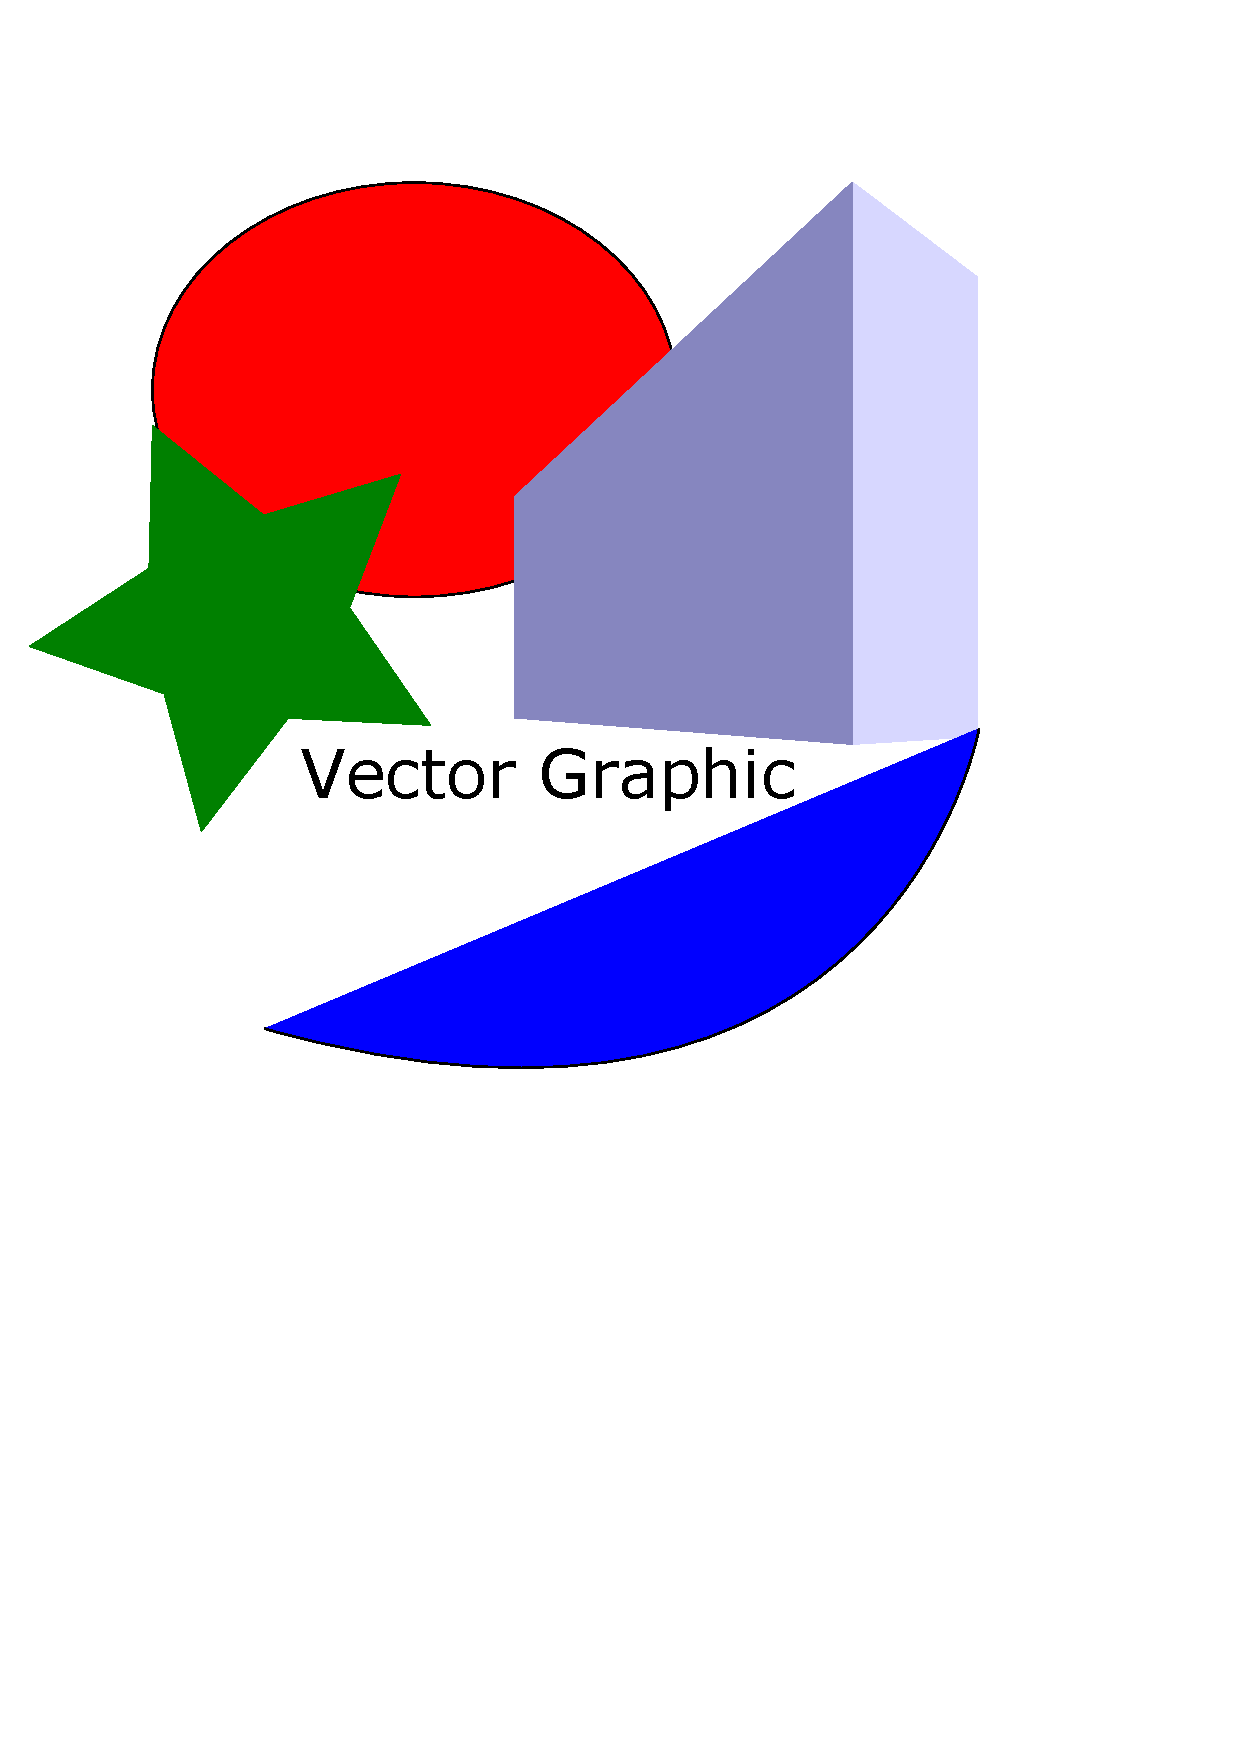
\includegraphics[width=0.40\textwidth]{figures/vectorGraphic.pdf}
	\caption{Example of a vector graphic}
	\label{fig:logo}
\end{figure}

Since this document is not the first and only one providing advice and hints regarding latex and structuring theses, the following chapter presents related work in this field.